\chapter{Evoluční algoritmy}
\section{Historie}
Začněme pohledem do historie Evolučních algoritmů na základě knih \citep{MitchellBook} a \citep{eibenIntro}. Darwinova myšlenka evoluce lákala vědce už před průlomem počítačů, Turing vyslovil myšlenku \textit{genetického a evolučního vyhledávání} už v roce 1948. V 50. a 60. letech nezávisle na sobě vznikají 4 hlavní teorie nesoucí podobnou myšlenku. Společným základem všech teorií byla evoluce populace kandidátů na řešení daného problému a jejich následná úprava způsoby hromadně nazývány jako genetické operátory, například mutace genů, přirozená selekce úspěšnějších řešení. \par 
Rechenberg a Schwefell (1965, 1973) představuje \textit{Evoluční strategie}, metoda optimalizující parametry v reálných číslech, jejich použití pro letadlová křídla. Fogel, Owens, Walsh zveřejňují \textit{evolutionary programming}(evoluční programování), technika využívající k reprezentaci kandidátů konečný automat(s konečným počtem stavů), který je vyvíjen mutací přechodů mezi stavy a následnou selekcí. \textit{Genetické algoritmy} vynalezl Holand v 60. letech a následně se svými studenty a kolegy z Michiganské Univerzity implementoval, oproti ES a EP nebylo hlavním cílem formovat algoritmus pro řešení konkrétních problémů, ale přenos obecného mechanismu evoluce jako metody aplikovatelné v informatickém světě. Princip GA spočívá v transformaci populace chromozonů(př. vektor 1 a 0) v novou populaci pomocí genetických operátorů křížení, mutací a inverze. V 1975 v knize \textit{Adaptation in Natural and  Artificial Systems} \citep{HolandBook} definoval genetický algoritmus jako abstrakci biologické evoluce spolu s teoretickým základem jejich používání. Ovšem někteří vědci používají pojem GA i ve významech hodně vzdálených původní Holandově definici. K sjednocení jednotlivých přístupů přispěl v 90. letehc Koza, dále jsou všechny zahrnuty jako oblasti \textit{Evolučních algoritmů}. Dnes existuje řada konferencí a odborných časopisů sdružující pracovníky zabývající se touto oblastí. Zmiňme ty větší z nich, co se týče konferencí: 
\href{http://gecco-2017.sigevo.org/index.html/HomePage}{GECCO}, \href{http://www.ppsn2016.org/conference}{PPSN}, 
\href{http://www.cec2017.org/}{CEC}, 
\href{http://www.evostar.org/2018/}{EVOSTAR}, 
časopisy: 
\href{http://www.mitpressjournals.org/loi/evco}{Evolutionary Computation}, 
\href{http://ieeexplore.ieee.org/xpl/RecentIssue.jsp?reload=true&punumber=4235}{IEEE Transactions on Evolutionary Computation}, 
\href{http://www.springer.com/computer/ai/journal/10710}{Genetic Programming and Evolvable Machines},
\href{https://www.journals.elsevier.com/swarm-and-evolutionary-computation/}{Swarm and Evolutionary Computation}
\section{Co je evoluční algoritmus?}
Ač existuje mnoho variant evolučních algoritmů, jak jsme zmínili v krátké pohledu do historie, spojuje je společná myšlenak populace jedinců uvnitř prostředí s omezenými podmínkami. Jedinci, jinak také nazývání kandidáti, soutěží o zdroje daného prostředí, tím je docíleno přírodní selekce(, přežijí jen Ti nejlepší). Pokud budeme mít k dispozici kvalitativní funkci, kterou se snažíme maximalizovat. Pak nebude problém vytvořit náhodné jedince z definičního oboru přesně této funkce. Náhodně vzniklé jedince můžeme ohodnotit, tímto způsobem dáme vzniku abstraktu pro měření fitness(, z anglického fit nejvíce vhodný). Z vzniklých a ohodnocených jedinců lze zvolit ty nejlepší pro tvorbu nové generace jedinců. Tvorba nové generace probíhá kombinováním zvolených rodičů a mutacemi jedinců. Jako kombinaci uvažujeme operátor, který je aplikován na 2-více zvolených kandidátů(, proto se jim také říká rodiče,) a tvořící 1-více nových jedinců(, také nazývány děti). Mutace je aplikována pouze na 1 jedince a její výsledkem je také pouze 1 jedinec. Tyto dvě operace aplikované na rodičovskou generaci vedou k vytvoření nových kandidátů(potomků,offsprings). I tato nová generace je ohodnocena fitness a dále soutěží se starými jedinci na základě fitness(, občas také v závislosti na stáří kandidáta,) o místo v nové generaci. Popsaný proces je opakován dokud není nalezen kandidát s dostatečně velkou fitness nebo narazíme na výpoční limit(, bylo dosaženo požadovaného počtu opakovaní apod). Základy Evolučního systému pohání 2 základní hnací síly: variační operátory, selektivní operátory. Variační operátory zajišťují potřebnou různorodost v populaci a tím tvoří nové cesty k úspěšnému kandidátovi. Oproti tomu selektivní operátory zvyšují průměrnou kvalitu řešení v celé populaci. Kombinací těchto operátorů obecně vede ke zlepšování fitness hodnot v následující generaci. Celkem jednodušše lze vidět, zda evoluce optimalizuje či nikoliv, stačí nám k tomu pozorovat zda se fitness v popolaci blíží více a více k optimálním hodnotám vzhledem k postupu v čase. Mnoho komponent zapříčiňuje, že EA se řadí ke stochastickým metodům, selekce nevybírá nejlepší jedince deterministicky i jedinci s malou fitness mají šanci být rodiči následující generace. Během kombinování jsou části rodičů , kterou budou z zkombinovány, také zvoleny náhodně. Podobně u mutací, část která bude změněna je taktéž určena náhodně, nové rysy nahrazující staré jsou generovány taktéž náhodně.  
\begin{center}
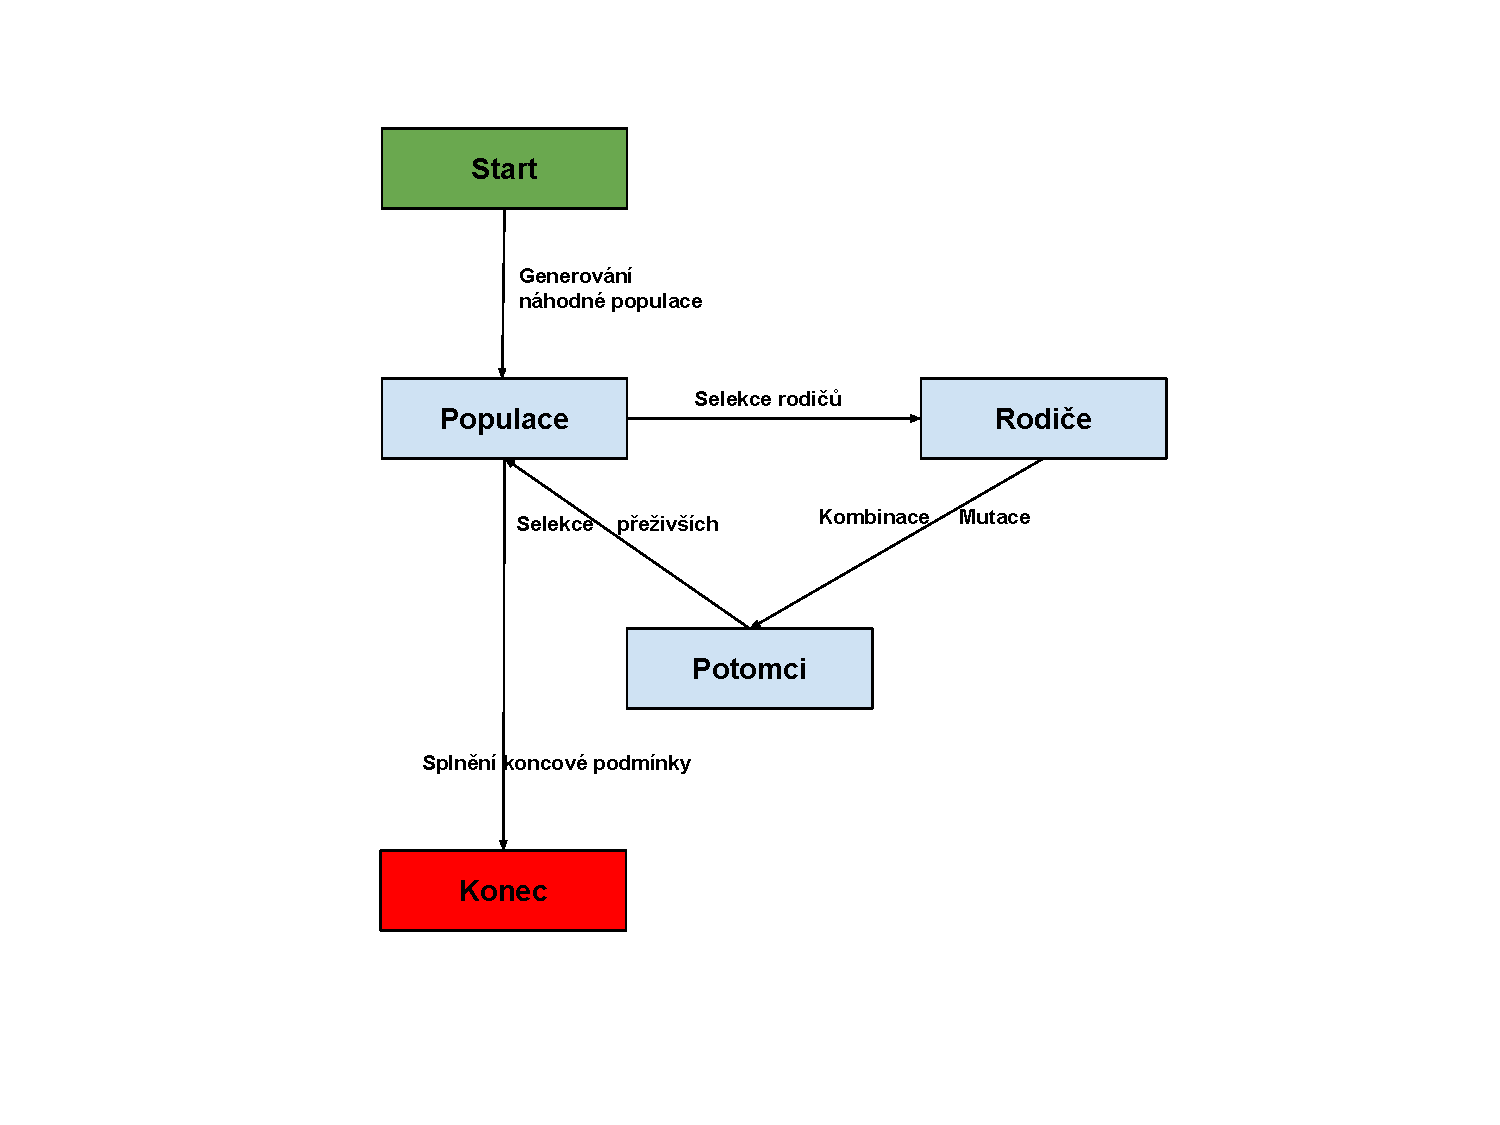
\includegraphics[scale=0.63]{../img/EA.pdf}
\end{center}
Ze schéma na obrázku můžeme vyčíst, že EA patří mezi algoritmy \"generate and test (vygeneruj a otestuj)\". Vyhodnocení fitness funkce poskytuje heuristický odhad kvality řešení, prohledávaní je řízen variací a selekcí. EA splňují charakteristické rysy G\&T algoritmů, zpracovávají zároveň celé kolekce kandidátů, většina EA míchá informace ze 2-více kandidátů a EA se řadí ke stochastickým metodám. \par
Různé dialekty evolučního programování, zmíněné v historickém okénku, splňují všechny tyto hlavní rysy a liší se pouze v technických detailech. Kandidáti jsou často reprezentování různě, liší se datové struktury pro jejich uchování i jejich zakódování. Typicky se jedná o řetězce nad konečnou abecedou v případě GA, vektory reálných čísel v ES, konečné automaty v EP a stromy v GP. Důvod těchto rozdílů je hlavně historický. Technicky však lze upřednostit jednu reprezentaci, pokud lépe odpovídá danému problému, tzn. kóduje kandidáta jednodušeji či přirozenější formou. Pro ilustraci zvolme řešení splnitelnosti(SAT) s n proměnnými, vcelku přirozeně sáhneme po použití řetězce bitů délky n a obsah i-tého bitu označuje, že i-tá proměnná má hodnotu (1)- pravda (0) - nepravda. Proto bychom použili jako vhodný EA Genetické Algortimy. Oproti tomu evoluce programu, který hraje šachy, by bylo vhodné použít derivační strom, kde by vrcholy odpovídali tahům na šachovnici. Přirozenější by tedy bylo použít GP. \par
Neopomeňme zmínit ještě dva důležité fakt. Za prvé kombinační a mutační operátory musí odpovídat dané reprezentaci, např. v GP kombinace pracuje se stromy(kombinuji podstromy..), zatímco v GA na řetězcích(prohazuji části řetězců). Za druhé oproti variacím musí fitness selekce záviset vždy pouze na fitness funkci, takže selekce pracuje nezávisle na reprezentaci.
\section{Části evolučních algoritmů}
Abychom vytvořili běhu schopný evoluční algoritmus, musíme specifikovat každou zmíněnou část a také inicializační funkci, která připraví první populaci. Pro konečný algoritmus ještě nesmíme opomenout a dodat koncovou podmínku. 
\begin{itemize}
\item{Reprezentace(definici individuí)}
\item{Ohodnocující funce(Fitness funce)}
\item{Populace}
\item{Selekce rodičů}
\item{Variační operátory(kombinace, mutace)}
\item{Selekce prostředí}
\end{itemize}
\subsection{Reprezentace}
Při tvorbě EA nejdříve musíme propojit prostor původního problému s prostorem řešení, kde se bude vlastní evoluce odehrávat. K docílení propojení je většinou potřeba zjednošit či vytvořit abstrakci nad aspekty reálného světa(prostor problému), abychom vytvořili vhodný prostor řešení, kde mohou být jednotlivá řešení ohodnocena. Neboli chceme docílit, aby možná řešení mohla být specifikována a uložena, tak aby s nimi mohl počítač pracovat. Objekty reprezentující možné řešení v kontextu původního problému jsou názývána \textbf{fenotyp}, zatímco kódování na straně EA prostoru \textbf{genotyp}. Reprezentace označuje mapování z fenotypů na genotypy, používá se ve významu funkci z fenotypu na genotyp(encode) i genotypu na fenotyp(decode) a předpokládá se, že pro každý genotyp existuje nejvýše jeden fenotyp. Například pro optimalizační problém, kde množinou řešení jsou celá čísla. Celá čísla tvoří množinu fenotypu a můžeme se rozhodnout pro reprezentaci v binárních číslech. Tedy 18 by byl fenotyp a 10010 jeho genotyp. Prostor fenotypů a genotypů se zpravidla velmi liší a celý proces EA se odehrává pouze v genotypovém prostoru, vlastní řešení dostanema rozkódováním nejlepšího genotypu po ukončení EA. Jelikož nevíme, jak vlastní řešení vypadá, je nanejvýš vhodné umět reprezentovat všechny možná řešení, v G\&T bychom řekli, že generátor je kompletní.
\begin{itemize}
\item V kontextu původního problému jsou následující výrazy ekvivaletní: fenotyp, kandidát(na řešení), jedinec, individuum (Množina všech možných řešení = fenotypový prostor)
\item V kontextu EA: getotyp, chromozon, jedinec, individuum (Množina kde probíhá EA prohledávání = genotypový prostor)
\item Části individuí jsou nazývány gen, locus, proměnná a dále se dělí na allely, či hodnoty
\end{itemize}
\subsection{Populace}
Populace je multimnožina genotypů, slouží jako jednotka evoluce. Populace utváří adaptaci a změny, zatímco vlastní jedinci se nijak nemění, jen vznikají nový a nahrazují předešlé. Pro danou reprezentaci je definice populace velmi jednoduchá charakterizuje ji pouze velikost. U některých specifických EA má populace další prostorové struktury, definované vzdáleností jedinců nebo relacemi sousedních jedinců. Což by se dalo připodobnit, reálným populacím, které se vyvíjejí v různých geografických prostředích. U většiny EA se velikost populace nemění, což vede k soutěživosti mezi jedinci(,zůstanou ti nejlepší). Na úrovni populací pracují právě selektivní operátory. Například zvolí nejlepší jedince aktuální populace jako rodiče následující, nahradí nejhorší jedince novými. Rozmanitost populace, vlastnost které chceme zpravidal docílit, je měřena jako počet různých řešení v multimnožině. Neexistuje však jediné hledisko podle, kterého lze tuto vlastnost měřit, většinou se používá počet rozdílných hodnot fitness, rozdílných fenotypů či genotypů a také například entropie(míra neuspořádanosti). Ovšem musíme mít na paměti, že jedna hodnota fitness v populaci neznamená, že populace obsahuje pouze jeden fenotyp, stejně tak jeden fenotyp nemusí odpovídat jednomu genotypu apod. 
\subsection{Selekce rodičů}
Rodičovská selekce, někdy také partnerská selekce, vybírá lepší jedince jako rodiče pro příští generaci. Jedinec se stává rodičem, pokud byl zvolen k aplikaci variačních operátorů a tím dal vzniknout novým potomkům. Společně s selekcí přeživších je rodičovská selekce zoodpovědná za zvedání kvality v populacích. Rodičovská selekce je v EA většinou pravděpodobnostní metoda, která dává jedincům s větší kvalitou mnohem větší šanci býti vybrán než těm nízkou. Nicméně i jedincům s nízkou kvalitou je často přidělena malá nenulová pravděpodobnost pro výběr, jinak by se celé prohledávání mohlo vydat slepou cestou a zaseknout se na lokální optimu. 
\subsection{Variační operátory}
Hlavní úlohou variačních operátorů(mutace, rekombinaci) je vytváření nových individuí ze starých. Z pohledu Generate  Test algoritmů spadají variační operátory do právě do Generate části. Obvykle je dělíme na dva typy podle jejich arity, jedná se o unární(Mutace) a n-arní(rekombinace) operátory.
\subsubsection{Mutace}
Ve většině případá myslíme unárním variačním operátorem mutace. Tento operátor je aplikován pouze na jeden genotyp a výsledkem je upravený potomek. Mutace řadíme mezi stochastické metody, výstup(potomek) totiž závisí na sérii náhodných rozhodnutí. Však mutace není vhodné pojmenování pro všechny variační operátory, například pokud se jedná o heuristiku závislou na daném problém, která se chová systematicky hledá slabé místo a následně se jej snaží vylepšit, nejedná se o mutaci v pravém slova smyslu. Obecně by mutace měla mutace způsobovat náhodné a nezaujaté změny. Unarní variační operátory hrají odlišnou roli v rozdílných EA opět díky historicky oddělenému vývoji. Zatímco v GP se nepoužívají vůbec, v GA má velmi důležitou roli a v EP se jedná o jediný variační operátor. Díky variačním operátorům aplikovaným v jednotlivých evolučních krocích dostává prohledávací prostor topologickou strukturu. Existují teorie formulící, že EA(s dostatečným časem) naleznou globální optimum daného problému opírající se právě o tuto topologii, spoléhají na vlastnost, že může vzniknout každý genotyp reprezentující možné řešení. Nejjednodušší cesta ke splnění těchto podmínek vede právě přes variační operátory. U mutací tohoto například dosáhneme, pokud povolíme, aby mohly skočit kamkoliv, tzn. každá allela může být zmutována na jakoukoli další s nenulovou pravděpodobností. Většina vědecká společnosti považuje tyto důkazy za nepříliš použitelné v praktickém využití a proto tuto vlastnost většina EA neimplementuje.  
\subsubsection{Rekombinace}
Rekombinace, také nazývána křížení, je binární variační operátor. Jak název napovídá, spojuje informace ze 2 rodičů(genotypů) do 1 nebo 2 potomků. Stejně jako mutace patří rekombinace k stochastickým operátorům. Rozhodnutí, jaké části budou zkombinovány a jakým způsobem tak bude docíleno závisí na náhodě. Role rekombinace se znovu liší v rozličných EA, v GP se jedná o jediné variační operátory, v EP nejsou použity vůbec. Rekombinační operátory s vyšší aritou(, používající více než 2 rodiče,) jsou možné a jednoduché na implementaci, dokonce několik studií potvrdilo, že mají velmi pozitivní vliv na celou evoluci, ale nemají tak hojné zastoupení, nejspíše proto, že neexistuje biologický ekvivalent. Rekombinace funguje na jednoduchém principu, slučuje 2 individua a může vyprodukovat potomky, které kombinují jejich výhodné vlastnosti, tedy potomek je úspěšnější než jeho rodiče. Tento princip podporuje fakt, že po 1000-letí se aplikací rekombinace na rostliny a zemědělská zvířata mnokrát podařilo vytvořit nové jedince s vyšším výnosem či jinými výhodnými vlastnostmy(odolnosti pro škůdcům,atd). Evoluční algoritmy vytváří množství potomků náhodnou rekombinací a doufáme, že zatímco malá část nové generace bude mít nežádoucí vlastnosti, většina se nezlepší ani si nepohorší a konečně další malá část předčí jejich rodiče. Na naší planetě se sexuálně(kombinací dvou jedinců) rozmnožují pouze vyšší organismy, což vzbuzuje dojem, že rekombinace je nejvyšší forma reprodukce. Neopomeňme, že  variační operátory jsou závislé na reprezentaci(genotypu) jedinců. Např. pro genotypy bitových řetězců může použít bitovou inverzi jako vhodný mutační operátor ovšem pokud bude genotyp strom musíme zvolit nějaký jiný. 
\subsubsection{Selekce prostředí}
Selekce prostředí, někdy také nazýváná selekce přeživších, jak název napovídá má blízko k selekci rodičů, odlišuje jednotlivá individua na základě jejich fitness hodnoty. Oproti rodičovské selekci ji však použiváme v jiné části evolučního cyklu, selekce prostředí spouštíme hned po vytvoření nových potomků. Jelikož velikost populace kandidátů bývá skoro vždy konstatní, tak je nutné rozhodnout které kandidáty zvolit do další generace. Toto rozhodnutí většinou závisí na fitnes kandidátů, také se však hledí na věk daného kandidáta(,generace v které vznikl). Na rozdíl od rodičovské selekce, která bývá stochastická, bývá selekce prostředí deterministickou metodou. Uveďme dvě nejběžnější metody, obě kladou největší důraz na fitness, první vybírá na nejlepší segment z množiny nových potomků i původní generace nezávisle, druhá dělá totéž jen z množiny nových potomků. Selekce prostředí je uváděna i pod názvem záměná strategie(replacement strategy), selekce prostředí(přeživších) se více používá pokud množina nových potomků je větší než velikost generace a záměna, když nových potomků je velmi málo.
\subsection{Jedinec}
Jedinec reprezentuje kandidáta na řešení problému. Může být reprezentován různými způsoby, např. v kontextu l-bitové vektory(GA), konečné automaty(EP), reálné vektory(ES). 
\subsection{Populace}
Populace označuje množinu jedinců.
\subsection{Generace}
Generace je populaci jednotlivého kroku EA.
\subsection{Fitness}
Fitness je funkce, která každému jedinci přiřadí reálné číslo, slouží k ohodnocení úspěšnosti kandidáta v kotextu řešeného problému. Pomocí EA se snažíme maximalizovat fitness v rámci další generace. Cíle EA je tedy nalézt jedince s nejvyšší fitness. 
\subsection{Kritérium ukončení}
Kritérium ukončení určuje koncovou podmínky pro ukončení prohledávání prostoru řešení. Většinou se jedná o počet generací, časový limit nebo dosáhnutí určité hodnoty fitness.  
\subsection{Základ EA}
Nejdříve se náhodně vygenerujeme inicializační populaci(P(0)), ohodnotíme jedince pomocí fitness funkce. Dokud není splněno koncové kritérium opakujeme následujíci algoritmus z P(t) vytvářej P(t+1). 
\begin{itemize}
    \item Výběr z rodičů 
    \item Rekombinace jedinců a jejich následná mutace, co odpovídá vzniku nových jedinců
    \item Ohodnocení nově vzniklých jedinců
    \item Enviromentální selekce ta vybere P(t+1) z P(t) a nově vzniklých jedinců
\end{itemize}
